\documentclass{article}
\usepackage{xeCJK}
\usepackage{amsmath}
\usepackage{algorithm}
\usepackage{algorithmic}
\usepackage{graphicx}

\setCJKmainfont{SimSun}
\renewcommand{\algorithmicrequire}{\textbf{Input:}}
\renewcommand{\algorithmicensure}{\textbf{Output:}}
\linespread{1.2}


\begin{document}
% \setlength{\parindent}{0pt}

一:
(1) \\
\[
dp[i][j] =  
\begin{cases}
    v_n * \lfloor{\frac{j}{w_n}}\rfloor \; , & i = n, \\
    dp[i + 1][j]\; , & 1 \leq j < w_i,\; 1 \leq i \leq n, \\
    \max{(dp[i + 1][j], dp[i][j - w_i] + v_i)}\; , & j \geq w_i,\; 1 \leq i \leq n, \\
\end{cases}
\]

(2) \\
\[
\begin{bmatrix}
0 & 2 & 4 & 6 & 8 & 10 \\
0 & 0 & 4 & 4 & 8 & 8 \\
0 & 0 & 0 & 4 & 5 & 5 \\
0 & 0 & 0 & 0 & 5 & 5 
\end{bmatrix}
\]

(3) \\
\begin{algorithm}
    \caption{\textbf{max\_value}}
    \label{alg:max_value}
    \begin{algorithmic}[1]
        \REQUIRE the weight array w, the value array v, the capacity c, the amount of items n
        \ENSURE the max value
        \STATE $dp[1...n][0...c]$
        \FOR{$j = 0$ to $c$}
        \STATE $dp[n][j] = v_n * (j // w_n)$
        \ENDFOR
        \FOR{$i = n - 1$ to $1$}
        \FOR{$j = 0$ to $c$}
        \IF{$j < w_i$}
        \STATE $dp[i][j] = dp[i + 1][j]$
        \ELSE
        \STATE $dp[i][j] = max(dp[i + 1][j], dp[i][j - w_i] + v_i)$
        \ENDIF
        \ENDFOR
        \ENDFOR
        \RETURN $dp[1][c]$
    \end{algorithmic}
\end{algorithm}
(4)\\
将二维数组降维至一维数组,伪代码如下:
\begin{algorithm}
    \caption{\textbf{max\_value2}}
    \label{alg:max_value2}
    \begin{algorithmic}[1]
        \REQUIRE the weight array w, the value array v, the capacity c, the amount of items n
        \ENSURE the max value
        \STATE $dp[0...c]$
        \FOR{$i = 1$ to $n$}
        \FOR{$j = w[i]$ to $c$}
        \STATE $dp[j] = max(dp[j], dp[j - w[i]] + v[i])$
        \ENDFOR
        \ENDFOR
        \RETURN $dp[c]$
    \end{algorithmic}
\end{algorithm}

\newpage
二.\\
设$E[i][j]$为$\{ k_i, \cdots, k_j\}$的优化解的期望搜索代价,\\
递推方程为
\[
E[i][j] = 
\begin{cases}
    q_{i - 1}, & j = i - 1 \\
    \underset{i \leq r \leq j}{min}(E[i][r -1] + E[r + 1][j] + W[i][j]), & j \geq i 
\end{cases}
\]
其中
\[
\begin{split}
W[i][j] = & \sum\limits_{m = i}^{r - 1}p_m + \sum\limits_{m = i - 1}^{r - 1}q_m \\
          & + \sum\limits_{m = i}^{j}p_m + \sum\limits_{m = i - 1}^{j}q_m + p_r
\end{split}
\]

计算可得最优二叉搜索树代价为$3.12$,结构为:
\begin{figure}[htbp]
    \centering
    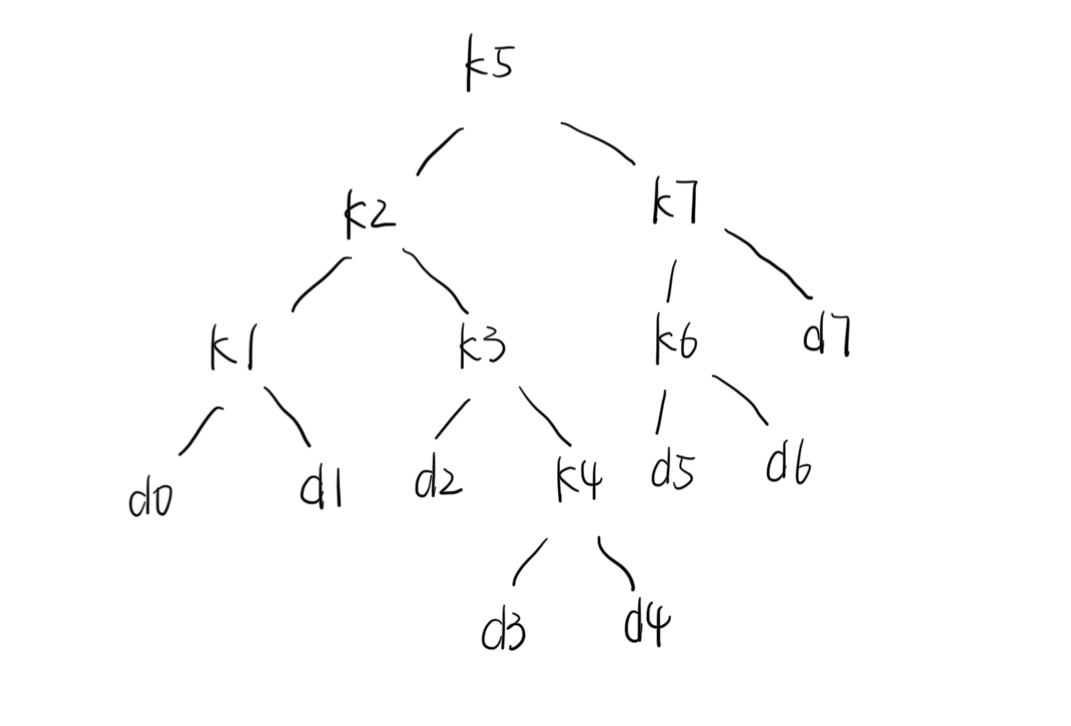
\includegraphics[width=1\textwidth, height=0.8\textwidth]{2.png}
    \caption{2.png}
    \end{figure} 
\newpage
三:\\
对于不首尾相连的情况,当前的第$i$个洞是否选取只取决于前面$i - 1$个洞是否选取,
比较第$i$个洞选取的收益和第$i - 1$个洞选取的收益并选择其中最优的即可。
设$m[i]$为前i个洞的最优解,则 \\
状态转移方程:
\[
m[i] = 
\begin{cases}
    nums[0], & i = 0 \\
    max(nums[0], nums[1]), & i = 1 \\
    max(m[i - 1], m[i - 2] + nums[i]), & 2 \leq i \leq n
\end{cases}
\]
对于首尾相连的情况,将$n$个洞分为$0~n-2$和$1~n-1$两组,即分别去掉
最后一个洞和第一个洞,最后在两种情况所求得的最优解中取最大值即可。

\end{document}